% !TeX root = ../main.tex

\chapter{长寿命粒子模型}

\section{物理背景}
长寿命粒子(Long Lived Particle, LLP)是指在探测器内衰变的时间尺度远大于标准模型粒子的寿命的粒子,它的存在是许多新物理模型的预言。
LLP长寿命的物理机制一般是由于它的衰变被禁戒或是被压低,其中压低可能出于衰变末态粒子的近退简并质量态(nearly-degenerate mass states)或是沟通LLP与末态粒子的相互作用为微弱的相互作用。
由于LLP具有较长的寿命、与标准模型粒子仅存在微弱的相互作用,因此它常被认为是暗物质的候选者。

由于LLP能在衰变前行进一定的宏观距离,其衰变产物不会从原始碰撞点(Primary Vertices)产生,而是在远离大多数标准模型粒子产生的初级顶点处形成一个次级顶点(Secondary Vertices),
该顶点也被称为偏离对撞顶点(Displaced Vertices)。
进一步,当LLP的衰变位置在电磁量能器之后时,其衰变产物会在电磁量能器内沉积少量能量,并且在其后的强子量能器内沉积绝大部分能量。
通过定义喷注在两类量能器中沉积的能量比值$\text{CalRatio}=E_{\text{H}}/E_{\text{EM}}$,可以鉴别LLP的衰变信号。\cite{calratio}

\begin{figure}[ht]
    \centering
    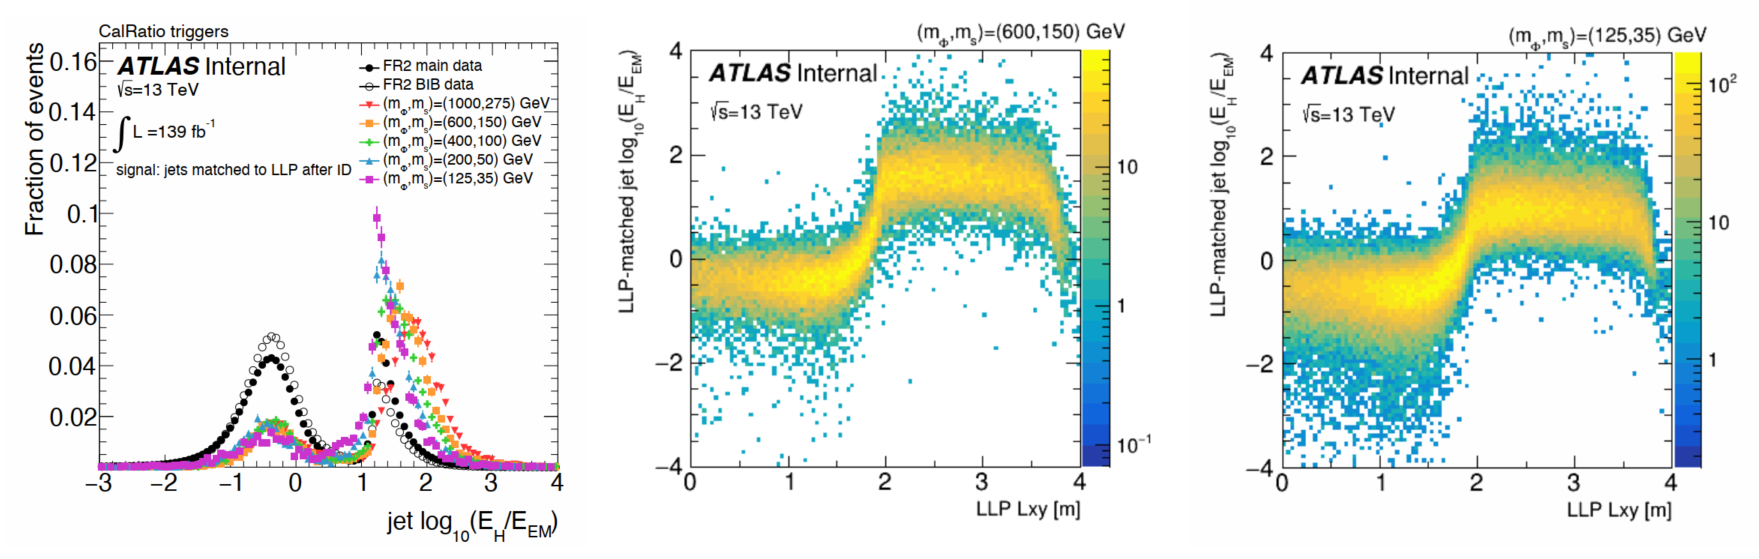
\includegraphics[width=\textwidth]{CalRatioDistribution.png}
    \caption{图号、图题置于图的下方}
    \label{fig:CalRatioDistribution}
    \figurenote{若有图注,图注置于图题下方。
        多个图注则须顺序编号,注序左缩进2字,与注文之间空一字符,续行悬挂缩进左对齐,两端对齐。
        注文的字数较少且是短语时,末尾不可加标点,多个图注可以在同一行通过自由选取字符空格将各个图注间隔开来;
        注文的字数较多或者甚至需要用句子说明时,该图注可以独立成行。
    }
\end{figure}


\section{具体模型}

\subsection{Hidden Sector 模型}

\subsection{超对称模型}

\subsection{Higgs-portal baryogenesis models}

